%% LyX 1.3 created this file.  For more info, see http://www.lyx.org/.
%% Do not edit unless you really know what you are doing.
\documentclass[twoside,english]{article}
\usepackage[T1]{fontenc}
\usepackage[latin1]{inputenc}
\usepackage{geometry}
\geometry{verbose,letterpaper,tmargin=1in,bmargin=1in,lmargin=1.25in,rmargin=1.25in}
\usepackage{fancyhdr}
\pagestyle{fancy}
\usepackage{array}
\usepackage{rotating}
\usepackage{graphicx}

\makeatletter

%%%%%%%%%%%%%%%%%%%%%%%%%%%%%% LyX specific LaTeX commands.
%% Bold symbol macro for standard LaTeX users
\newcommand{\boldsymbol}[1]{\mbox{\boldmath $#1$}}

%% Because html converters don't know tabularnewline
\providecommand{\tabularnewline}{\\}

\usepackage{babel}
\makeatother
\begin{document}

\title{\textbf{Coordinate Systems in the Goddard Mission Analysis Tool (GMAT)}}


\author{{\normalsize Darrel J. Conway}\\
{\normalsize Thinking Systems, Inc.}\\
{\normalsize 6441 N Camino Libby}\\
{\normalsize Tucson, AZ 85718}}

\maketitle
\begin{center}\textbf{Design Document}\end{center}

\begin{abstract}
This document presents design guidelines for the coordinate system
classes in the Goddard Mission Analysis Tool (GMAT). It describes
how the GMAT software implements the coordinate system math described
in the GMAT Mathematical Specifications\cite{GmatMathSpec}. This
description includes the initial design for the classes that provide
coordinate system support in GMAT. The interactions between these
classes and the rest of the GMAT system are also described.
\end{abstract}

\section{Introduction}

The Goddard Mission Analysis Tool (GMAT) is a multi-platform orbit
simulator designed to support multiple spacecraft missions flying
anywhere in the solar system. GMAT is written in C++ and runs on Windows,
Macintosh and Linux computer systems. The tool provides an integrated
interface to MATLAB, a high level computing environment from the Mathworks,
Inc\cite{MATLAB}. The GMAT graphical user interface (GUI) is written
using the wxWidgets GUI Toolkit\cite{wxWidgets}, an open source library
that compiles and runs under all of the target operating systems. 

GMAT is an object-oriented system, using the full extent of the C++
language to implement the object model that provides GMAT's functionality.
The first three builds of GMAT provided capabilities to model orbits
in the vicinity of the Earth, including detailed force modeling, impulsive
maneuvers, and parameter targeting using a differential corrector.
All of these capabilities can be controlled either using either the
GMAT graphical user interface or a custom scripting language designed
to simplify GMAT and MATLAB interactions. The fourth build of the
system generalizes the capabilities of GMAT modeling for other orbital
regimes. 

In order to model spacecraft trajectories in these regimes, GMAT needs
to be able to represent the spacecraft state and related quantities
in coordinate systems that are convenient to each regime. This document
describes how these coordinate systems are implemented in the GMAT
code.


\section{\label{sec:CSClassDescription}Coordinate System Classes}

Figure \ref{figure:HighLevelCSClasses} shows the core C++ classes
(drawn using Poseidon\cite{Poseidon}) added to GMAT to provide support
for coordinate systems in Build 4. The coordinate system capabilities
are provided by the incorporation of these classes into the GMAT base
subsystem%
\footnote{The GMAT code base consists of a set of classes that provide the core
functionality of the system, the {}``base'' subsystem, and classes
that comprise the graphical user interface, the {}``gui'' subsystem.
All of the classes described in this document are members of the base
subsystem, with the exception of the recommendations for changes to
the panels on the GUI.%
}.

%
\begin{figure}
\centerline{\fbox{\includegraphics[%
  clip,
  scale=0.6]{./graphics/HighlevelCSclasses.jpg}}}


\caption{\label{figure:HighLevelCSClasses}Coordinate System Classes in GMAT}
\end{figure}


The coordinate system classes consist of a CoordinateSystem class
that acts as the interface between the conversions and the rest of
GMAT, an AxisSystem base class with a derived hierarchy used for rotational
conversions, a CoordinateConverter class that manages conversions
between different coordinate systems, and a factory constructed as
a singleton that create the AxisSystem objects. The CoordinateSystem
class is the component that is instantiated when a user {}``Creates''
a coordinate system object. 

Previous builds of GMAT included classes that model spacecraft, formations,
and celestial objects. These classes were derived from a core base
class named GmatBase. A new intermediate class, SpacePoint, is implemented
in GMAT to make access to position, velocity, and rotational data
available to the coordinate system classes when needed. Section \ref{sub:SpacePointClassDescription}
describes this class.


\subsection{The CoordinateSystem Class}

The CoordinateSystem class is a configured component that implements
the functionality needed to convert into and out of a specified coordinate
system. Internally, GMAT performs computations in a Mean of J2000
Earth Equatorial coordinate system, centered at one of the celestial
bodies in the GMAT solar system (i.e. the Sun, a planet, or a moon)
or at a barycenter or libration point. Each CoordinateSystem instance
provides methods to transform into and out of these J2000 coordinate
systems. It contains the data necessary for translation calculations,
along with a member object pointer that is set to an AxisSystem instance
for coordinate systems whose principle axes are not parallel to the
Mean of J2000 Earth Equatorial axes, or to NULL for coordinate systems
that are oriented parallel to these axes. 

The AxisSystem class provides the methods needed to rotate the coordinate
system into and out of the Mean of J2000 Earth Equator frame. The
AxisSystem is set for a given CoordinateSystem by setting the axes
member to an AxisSystem instance. 

GMAT uses a late binding scheme to provide interconnections between
objects used when modeling an analysis problem. Individual components
are configured from either the grapical user interface or a script
file describing the objects that need to be modeled. Connections between
these objects are defined using the names of the objects, but the
actual object instances used in the model are not set until the simulation
is run. Upon execution, the configured objects are copied into the
analysis workspace, called the Sandbox, and the connections between
the configured objects are established immediately prior to the run
of the simulation. The Initialize method in the CoordinateSystem class
implements this late binding for the connection between the coordinate
system instance and the related SpacePoints.


\subsection{The AxisSystem Class Hierarchy}

GMAT is capable of supporting numerous coordinate system orientations.
These orientations are defined through the AxisSystem class; each
unique axis orientation is implemented as a separate class derived
from the AxisSystem base class. Figure \ref{figure:AxisSystemOverview}
shows an overview of the AxisSystem class hierarchy, and identifies
the top level classes in this hierarchy.

%
\begin{figure}
\centerline{\fbox{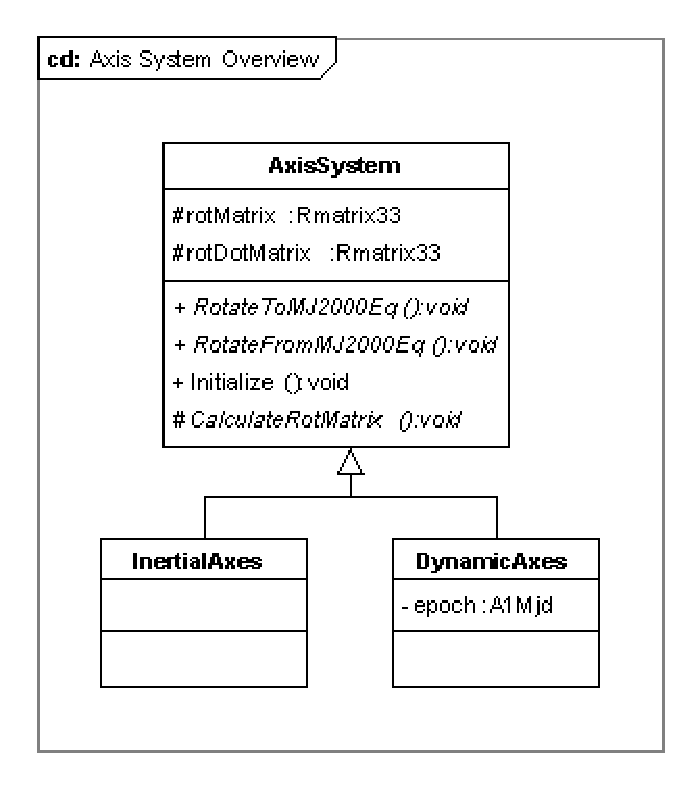
\includegraphics[%
  clip,
  scale=0.6]{./graphics/AxisSystemOverview.jpg}}}


\caption{\label{figure:AxisSystemOverview}Top level AxisSystem Derived Classes}
\end{figure}


The orientations of the coordinate systems in GMAT fall into two broad
categories: axes that change orientation over time, and those that
remain fixed in orientation. The latter category requires computation
of the rotation matrices one time, at initialization, in order to
perform the rotations into and out of the coordinate system. Figure
\ref{figure:InertialAxisHierarchy} shows the six inertial axis systems
supported in GMAT. These systems support equatorial and ecliptic versions
of Mean of J2000, Mean of Epoch, and True of Epoch transformations.

%
\begin{figure}
\centerline{\fbox{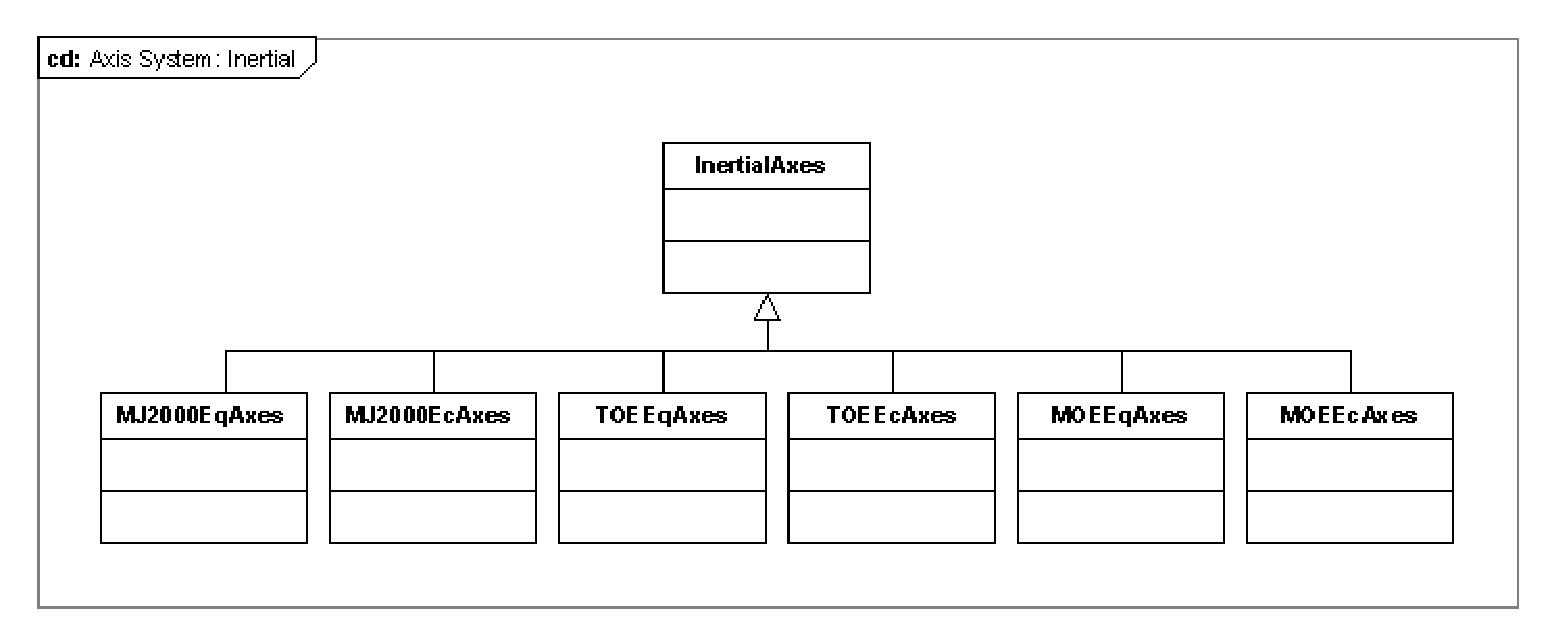
\includegraphics[%
  clip,
  scale=0.6]{./graphics/AxisSystemInertial.jpg}}}


\caption{\label{figure:InertialAxisHierarchy}Inertial Axis Classes}
\end{figure}


Coordinate systems that are not fixed in orientation over time are
derived from the DynamicAxes class, as is shown in Figure \ref{figure:DynamicAxisHierarchy}.
These coordinate systems include equatorial and ecliptic versions
of the mean of date and true of date axes, along with axes that evolve
with the polar motion of the body's rotational axis (implemented in
the EquatorAxes class) and axes that are fixed on the body's prime
meridian (the BodyFixedAxes class). All of these classes require recomputation
of the orientation of the axes as the epoch of the model evolves.

%
\begin{figure}
\centerline{\fbox{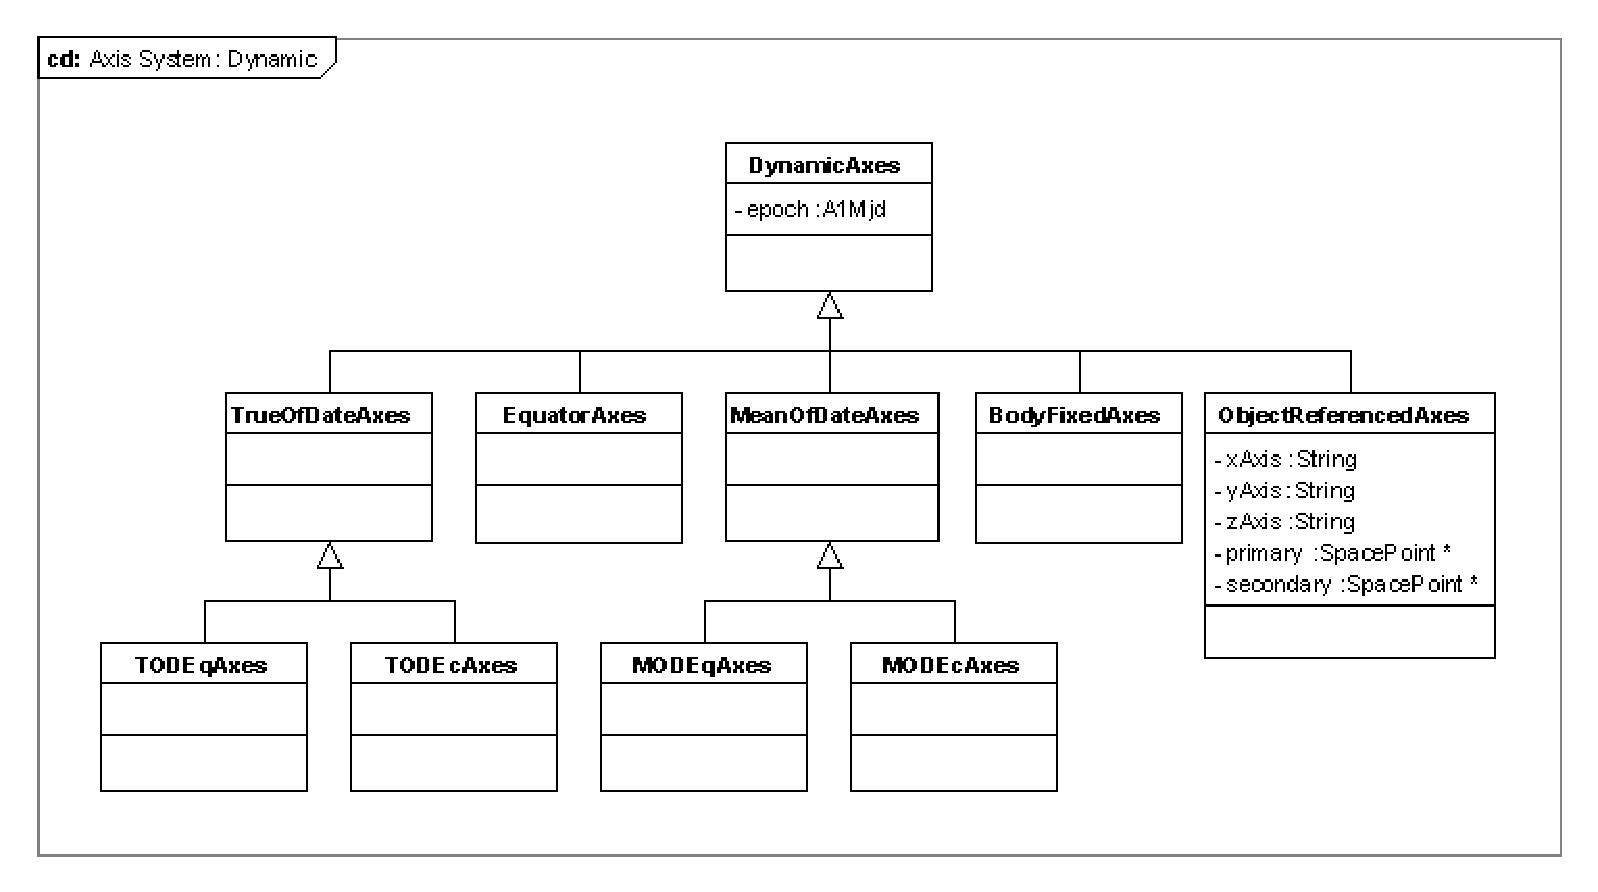
\includegraphics[%
  clip,
  scale=0.6]{./graphics/AxisSystemDynamic.jpg}}}


\caption{\label{figure:DynamicAxisHierarchy}Dynamic Axis Classes}
\end{figure}


One additional class in Figure \ref{figure:DynamicAxisHierarchy}
bears discussion here. GMAT supports numerous coordinate systems that
reference bodies that are not celestial objects -- specifically coordinate
systems that use Lagrange points, barycenters, spacecraft, and formations
to define the coordinate origins and axes. These coordinate systems
use the ObjectReferencedAxes class to construct the coordinate basis
and rotation matrices. The GMAT Mathematical Specifications\cite{GmatMathSpec}
provide detailed descriptions of how this class operates.


\subsection{CoordinateSystem and AxisSystem Collaboration}

The GMAT Mathematical Specification\cite{GmatMathSpec} includes a
flow chart that describes the process of transforming between coordinate
systems. This process is performed in the GMAT code using the CoordinateConverter
class and the public methods of the CoordinateSystem class. When GMAT
needs a conversion from one coordinate system to another, the method
\texttt{CoordinateConverter::Convert} is called with the epoch, input
state, input coordinate system, output state, and output coordinate
system as parameters. The converted state vector is stored in the
output state parameter.

The Convert method calls the conversion method \texttt{CoordinateSystem::ToMJ2000Eq}
on the input coordinate system, followed by \texttt{CoordinateSystem::FromMJ2000Eq}
on the output coordinate system. \texttt{ToMJ2000Eq} calls the \texttt{AxisSystem::RotateToMJ2000Eq}
method followed by the \texttt{Coordinate\-System::TranslateToMJ2000Eq}
method, converting the input state from the input coordinate system
into Mean of J2000 Equatorial coordinates. Similarly, \texttt{FromMJ2000Eq}
calls the \texttt{Coordinate\-System::TranslateFromMJ2000Eq} method
and then the \texttt{AxisSystem::RotateFromMJ2000Eq} method, converting
the intermediate state from Mean of J2000 Equatorial coordinates into
the output coordinate system, completing the transformation from the
input coordinate system to the output coordinate system. Each of the
conversion routines takes a SpacePoint pointer as the last parameter
in the call. This parameter identifies the J2000 coordinate system
origin to the conversion routine. If the pointer is NULL, the origin
is set to the Earth.

The following paragraphs provide programmatic samples of these conversions.


\subsubsection{Code Snippets for a Conversion}

Figure \ref{figure:TransformDetails}, generalized from the GMAT mathematical
specification, illustrates the procedure used to implement a transformation
from one coordinate system to another. The following paragraphs provide
code snippets with the corresponding function arguments for this process.

%
\begin{figure}
\centerline{\fbox{\includegraphics[%
  clip,
  scale=0.6]{./graphics/ConversionDetails.jpg}}}


\caption{\label{figure:TransformDetails}GMAT Procedure for a Generic Coordinate
Transformation}
\end{figure}


When GMAT needs to convert from one coordinate system to another,
this method is called:

\begin{quotation}
\texttt{if (!coordCvt->Convert(epoch, instate, inputCS, outstate,
outputCS))}

\texttt{~~~throw CoordinateSystemException({}``Conversion from
''}

\texttt{~~~~~~+ inputCS->GetName() + {}`` to '' + outputCS->GetName()
+ {}`` failed'');}
\end{quotation}
This method invokes the calls listed above, like this:

\begin{quotation}
\texttt{// Code in CoordinateConverter::Convert}

\texttt{if (!inputCS->ToMJ2000Eq(epoch, instate, internalState, J2000Body))}

\texttt{~~~throw CoordinateSystemException({}``Conversion to MJ2000
failed for ''}

\texttt{~~~~~~+ inputCS->GetName());}~\\


\texttt{if (!outputCS->FromMJ2000Eq(epoch, internalState, outState,
J2000Body))}

\texttt{~~~throw CoordinateSystemException({}``Conversion from
MJ2000 failed for ''}

\texttt{~~~~~~+ outputCS->GetName());}
\end{quotation}
The conversion code from the input state to Mean of J2000 Equatorial
Coordinates is accomplished using the calls

\begin{quotation}
\texttt{// Code in CoordinateSystem::ToMJ2000Eq}

\texttt{if (axes)~~~~~~// axes == NULL for MJ2000Eq orientations}

\texttt{~~~if (!axes->RotateToMJ2000Eq(epoch, instate, internalState,
J2000Body))}

\texttt{~~~~~~throw CoordinateSystemException({}``Rotation
to MJ2000 failed for ''}

\texttt{~~~~~~~~~+ instanceName);}

\texttt{else~~~~~~~~~~~// Set the intermediate state to
the input state}

\texttt{~~~internalState = instate;}\\


\texttt{if (!TranslateToMJ2000Eq(epoch, internalstate, internalState,
J2000Body))}

\texttt{~~~throw CoordinateSystemException({}``Translation to
MJ2000 failed for '' }

\texttt{~~~~~~+ instanceName);}
\end{quotation}
and the conversion from Mean of J2000 Equatorial Coordinates to the
output state is performed using these calls:

\begin{quotation}
\texttt{// Code in CoordinateSystem::FromMJ2000Eq}

\texttt{if (!TranslateFromMJ2000Eq(epoch, internalstate, internalState,
J2000Body))}

\texttt{~~~throw CoordinateSystemException({}``Translation from
MJ2000 failed for ''}

\texttt{~~~~~~+ instanceName);}~\\


\texttt{if (axes)~~~~~~// axes == NULL for MJ2000Eq orientations}

\texttt{~~~(!axes->RotateFromMJ2000Eq(epoch, internalState, outstate,
J2000Body))}

\texttt{~~~~~~throw CoordinateSystemException({}``Rotation
from MJ2000 failed for ''}

\texttt{~~~~~~~~~+ instanceName);}

\texttt{else~~~~~~~~~~~// Set the output state to the intermediate
state }

\texttt{~~~outstate = internalState;}
\end{quotation}

\subsection{\label{sub:SpacePointClassDescription}The SpacePoint Class}

In general, coordinate systems are defined in reference to locations
and directions in space. Many of the coordinate systems used in GMAT
have the direction fixed based on an external reference -- for example,
the MJ2000Eq system has the z-axis pointed along the Earth's rotation
axis at the J2000 epoch and the x-axis aligned with the vernal equinox
at the same epoch. GMAT also supports coordinate systems constructed
in reference to objects internal to the GMAT -- typically a planet,
the Sun, a moon, or a spacecraft can be used, as can special points
in space like Lagrange points or the barycenter of a multi-body system.
The coordinate system classes need to be able to access position and
velocity data about these objects in a generic fashion. GMAT has a
class, SpacePoint, that provides this access. SpacePoint is the base
class for all of the objects that model location data in the solar
system, as is shown in Figure~\ref{figure:SpacePointHierarchy}.

%
\begin{figure}
\centerline{\fbox{\includegraphics[%
  clip,
  scale=0.6]{./graphics/SpacePoint.jpg}}}


\caption{\label{figure:SpacePointHierarchy}The SpacePoint Class Hierarchy}
\end{figure}



\section{\label{sec:CSScriptConfiguration}Configuring Coordinate Systems}


\subsection{Scripting a Coordinate System}

The script commands used to create a coordinate system object in GMAT
are defined in the GMAT Mathematical Specifications\cite{GmatMathSpec}.
Coordinate System scripting is performed using the following lines
of script:

\begin{quotation}
\texttt{Create CoordinateSystem csName}

\texttt{GMAT csName.Origin = <SpacePoint name>;}

\texttt{GMAT csName.Axes = <Axis type>;}

\texttt{GMAT csName.Primary = <Primary SpacePoint name, if needed>;}

\texttt{GMAT csName.Secondary = <Secondary SpacePoint name, if needed>;}

\texttt{GMAT csName.Epoch.<Format> = <Epoch data, if needed>;}

\texttt{\% Only two of these three can exist for a given coordinate }

\texttt{\% system; see Table \ref{table:CSParms} for more information}

\texttt{GMAT csName.XAxis = <$\pm$R, $\pm$V, or $\pm$N>;}

\texttt{GMAT csName.YAxis = <$\pm$R, $\pm$V, or $\pm$N>;}

\texttt{GMAT csName.ZAxis = <$\pm$R, $\pm$V, or $\pm$N>;}
\end{quotation}
The fields in angle brackets are used to set the parameters that define
the coordinate system. Table~\ref{table:CSParms} provides a brief
description of these fields; more details are available in \cite{GmatMathSpec}.

%
\begin{table}

\caption{\label{table:CSParms}Coordinate System Parameters}

\begin{center}\begin{tabular}{|p{0.8in}|p{0.9in}|p{1.3in}|p{2.5in}|}
\hline 
Parameter&
Required/ Optional&
Allowed Values&
Description\tabularnewline
\hline
\hline 
Origin&
Required&
\begin{flushleft}Any Named SpacePoint\end{flushleft}&
Defines the location of the coordinate system origin.\tabularnewline
\hline 
Axes&
Required&
\begin{flushleft}Equator, MJ2000Ec, MJ2000Eq, TOEEq, MOEEq, TODEq,
MODEq, TOEEc, MOEEc, TODEc, MODEc, Fixed, ObjectRefernced\end{flushleft}&
Defines the orientation of the coordinate axes in space.\tabularnewline
\hline 
Primary&
Optional&
\begin{flushleft}Any Named SpacePoint\end{flushleft}&
Defines the primary body used to orient axes for systems that need
a primary body.\tabularnewline
\hline 
Secondary&
Optional&
\begin{flushleft}Any Named SpacePoint\end{flushleft}&
Defines the secondary body used to orient axes for systems that need
a secondary body.\tabularnewline
\hline 
Epoch&
Optional&
Any GMAT Epoch&
Sets the reference epoch for systems that need a reference epoch.\tabularnewline
\hline 
XAxis&
Optional&
$\pm\textrm{R,}\pm\textrm{V,}\pm\textrm{N}$&
Used for ObjectReferences axes only; two of the three axes are set,
and one must reference $\pm N$.\tabularnewline
\hline 
YAxis&
Optional&
$\pm\textrm{R,}\pm\textrm{V,}\pm\textrm{N}$&
Used for ObjectReferences axes only; two of the three axes are set,
and one must reference $\pm N$.\tabularnewline
\hline 
ZAxis&
Optional&
$\pm\textrm{R,}\pm\textrm{V,}\pm\textrm{N}$&
Used for ObjectReferences axes only; two of the three axes are set,
and one must reference $\pm N$.\tabularnewline
\hline
\end{tabular}\end{center}
\end{table}


In the following paragraphs, the interactions between the script interpreter
subsystem and the coordinate system classes are described.


\subsubsection{Script Interpreter Actions}

In GMAT, the ScriptInterpreter reads each line of script and sets
up the corresponding objects. The lines of script above map to calls
made in the ScriptInterpreter code, as described in the following
text. 

The Create line causes the ScriptInterpreter to call the CoordinateSystemFactory
and requests a CoordinateSystem instance:

\begin{quotation}
\texttt{// In the Interpreter subsystem}

\texttt{GmatBase {*}csInstance =}

\texttt{~~~moderator->CreateCoordinateSystem({}``CoordinateSystem'',
{}``csName'');}
\end{quotation}
The resulting coordinate system is registered with the configuration
manager.

The Origin line sets the originName parameter on this instance:

\begin{quotation}
\texttt{// First determine that the parm is a string}

\texttt{Gmat::ParameterType type = csInstance->GetParameterType({}``Origin'');}

\texttt{// Here type is a string, so this is called:}

\texttt{csInstance->SetStringParameter({}``Origin'', <SpacePoint
name>);}
\end{quotation}
The Axes line creates an instance of the AxisSystem and passes it
to the coordinate system:

\begin{quotation}
\texttt{// First determine that the parm is an internal object}

\texttt{Gmat::ParameterType type = csInstance->GetParameterType({}``Axes'');}

\texttt{// Here type is an object, so this is called:}

\texttt{GmatBase {*}axesInstance = moderator->CreateAxisSystem(<Axis
type>, {}``'');}

\texttt{// Then the object is set on the coordinate system}

\texttt{csInstance->SetRefObject(axesInstance);}
\end{quotation}
The Primary line sets the primary body on the AxisSystem instance.
This is done by passing the data through the CoordinateSystem object
into the AxisSystem object:

\begin{quotation}
\texttt{// First determine that the parm is a string}

\texttt{Gmat::ParameterType type = csInstance->GetParameterType({}``Primary'');}

\texttt{// Pass the string to the coordinate system}

\texttt{csInstance->SetStringParameter({}``Primary'', <SpacePoint
name>);}~\\


\texttt{...}\\


\texttt{// In CoordinateSystem, this parameter is passed to the AxisSystem:}

\texttt{axes->SetStringParameter({}``Primary'', <SpacePoint name>);}
\end{quotation}
The Secondary line is treated similarly to the primary line:

\begin{quotation}
\texttt{// First determine that the parm is a string}

\texttt{Gmat::ParameterType type = csInstance->GetParameterType({}``Secondary'');}

\texttt{// Pass the string to the coordinate system}

\texttt{csInstance->SetStringParameter({}``Secondary'', <SpacePoint
name>);}~\\


\texttt{...}\\


\texttt{// In CoordinateSystem, this parameter is passed to the AxisSystem:}

\texttt{axes->SetStringParameter({}``Secondary'', <SpacePoint name>);}
\end{quotation}
The Epoch line is handled like in the Spacecraft object, and the XAxis,
YAxis and ZAxis lines are treated as string inputs, like the Primary
and Secondary lines, above. 


\subsection{Default Coordinate Systems}

GMAT defines several coordinate systems by default when it is initialized.
These systems are listed in Table \ref{table:DefaultCSs}.

%
\begin{table}

\caption{\label{table:DefaultCSs}Default Coordinate Systems defined in GMAT}

\centerline{\begin{tabular}{|p{1in}|p{1in}|p{1.5in}|p{2in}|}
\hline 
Name&
Origin&
Axis System&
Comments\tabularnewline
\hline
\hline 
EarthMJ2000Eq&
Earth&
MJ2000 Earth Equator&
The default coordinate system for GMAT\tabularnewline
\hline 
EarthMJ2000Ec&
Earth&
MJ2000 Ecliptic&
\tabularnewline
\hline 
EarthFixed&
Earth&
Body Fixed&
The Earth fixed system is used by the gravity model for full field
modeling\tabularnewline
\hline 
BodyFixed&
Other celestial bodies&
Body Fixed&
Fixed systems used by the gravity model for full field modeling at
other bodies\tabularnewline
\hline
\end{tabular}}
\end{table}



\section{Coordinate System Integration }

Sections \ref{sec:CSClassDescription} and \ref{sec:CSScriptConfiguration}
describe the internal workings of the GMAT coordinate systems, but
do not explain how the coordinate system code interacts with the rest
of GMAT. This section outlines that information.


\subsection{General Considerations}

GMAT uses coordinate systems in several general areas: for the input
of initial state data, internally in the impulsive and finite burn
code, force models and propagation code, in the calculation of parameters
used to evaluate the behavior of the model being run, and in the graphical
user interface (GUI) to display data as viewed from a coordinate system
based perspective.


\subsection{Creation and Configuration}


\subsubsection{Coordinate System Creation}

Coordinate systems are created through a series of interactions between
the GMAT interpreters, the Moderator, and the Factory system. Figure
\ref{figure:CSCreationSequence} shows the sequence followed by the
ScriptInterpreter when a coordinate system is configured from a script.
The procedure is similar when the GUI configures a coordinate system,
with one exception. The ScriptInterpreter translates a script file
a line at a time, so it needs to look up the CoordinateSystem object
each time it is referenced in the script. The GUI configures the coordinate
system from a single panel, so the coordinate system object does not
need to be found each time a parameter is accessed.

%
\begin{figure}
\centerline{\fbox{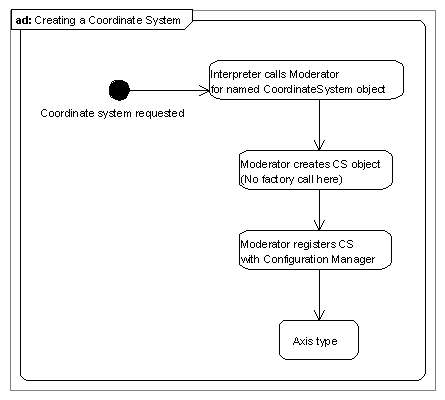
\includegraphics[%
  clip,
  scale=0.5]{/home/djc/latex/GmatDesignDocs/graphics/CSCreationSequence.jpg}}}


\caption{\label{figure:CSCreationSequence}Coordinate System Creation and
Configuration Sequence}
\end{figure}



\subsubsection{Startup Considerations}

When a user starts GMAT, the executable program creates a singleton
instance of the Moderator. The Moderator is the core control module
in GMAT; it manages the creation and deletion of resources, the interfaces
between the core components of the system and the external interfaces
(including the GUI and the scripting engines), and the execution of
GMAT simulations. When the Moderator is created, it creates a variety
of default resources, including the default factories used to create
the objects in a simulation. The factories that get created include
the CoordinateSystemFactory.

After it has created the factories and constructed the default solar
system, the Moderator creates the default coordinate systems listed
in Table \ref{table:DefaultCSs}, following a procedure like the one
shown in Figure \ref{figure:CSCreationSequence}. These coordinate
systems are registered with the Configuration Manager using the names
in the table. Users can use these coordinate systems without any taking
any additional configuration actions.


\subsection{Sandbox Initialization}

When a user runs a mission sequence, the Moderator takes the following
sequence of actions%
\footnote{The description here references a Sandbox for the run. The Moderator
can be configured to manage a collection of Sandboxes; in that case,
the actions described here are applied to the current Sandbox from
that collection.%
}:

\begin{enumerate}
\item Send the current SolarSystem to the Sandbox for cloning
\item Load the configured objects one at a time into the Sandbox. These
objects are cloned%
\footnote{The current build of GMAT does not fully implement cloning for the
configured objects. This issue is being corrected.%
} into the Sandbox.
\item The Sandbox is initialized.
\item The Mission is executed.
\end{enumerate}
The critical piece for successful execution of a GMAT mission is the
third step. When the Sandbox is initialized, the following actions
are executed:

\begin{enumerate}
\item The local solar system object is set for all of the objects that need
it.
\item Reference object pointers are set on objects that use them.
\item \label{enu:ObjectInit}The objects are initialized.
\item Parameters are configured.
\item The command sequence is configured.

\begin{enumerate}
\item The object table is passed to each command.
\item The solar system is passed to each command.
\item \label{enu:CS-CommandInit}The command is initialized.
\end{enumerate}
\end{enumerate}
The coordinate system objects are fully initialized and ready for
use by the end of the step \ref{enu:ObjectInit}. Commands that use
the coordinate system objects have the object associations set in
step \ref{enu:CS-CommandInit}.


\subsection{Initial States}

Users need to set the locations and initial motion of spacecraft,
ground stations, and other physical entities modeled in GMAT using
a coordinate system that makes this data simple to specify. For this
reason, GMAT lets users select all or a portion of the coordinate
system needed for these objects.


\subsubsection{Spacecraft}

The initial state for a spacecraft is expressed as an epoch and six
numerical quantities representing the spacecraft's location and instantaneous
motion. These quantities are typically expressed as either six Cartesian
elements -- the x, y, and z components of the position and velocity,
six Keplerian elements -- the semimajor axis, eccentricity, inclination,
right ascension of the ascending node, argument of pariapsis, and
the anomaly in one of three forms (true, mean, or eccentric), or one
of several other state representations. The element representation
depends on the coordinate system used. Some representations cannot
be used with some coordinate systems -- for example, the Keplerian
representation requires a gravitational parameter, $\mu=GM$, in order
to calculate the elements, so coordinate systems that do not have
a massive body at the origin cannot be used for Keplerian elements.
For these cases, GMAT reports an error if the element type is incompatible
with the coordinate system.


\subsubsection{Ground Stations and Other Body Fixed Objects}

Ground station objects and other objects connected to physical locations
on a body are expressed in terms of the latitude, longitude, and height
above the mean ellipsoid for the body. The coordinate system used
for these objects is a body fixed coordinate system. Users can specify
the central body when they configure these objects. The body radius
and flattening factor for that body are used to calculate the mean
ellipsoid. Latitude is the geodetic latitude of the location, and
longitude is measured eastwards from the body's prime meridian. 

GMAT does not currently support ground stations or other body fixed
objects. This section will be updated when this support is added to
the system.


\subsection{Forces and Propagators}

Internal states in GMAT are always stored in a Mean of J2000 Earth-Equator
coordinate system. The origin for this system is set to either a celestial
body (i.e. the Sun, a planet, or a moon), a barycenter between two
or more bodies, or a Lagrange point. The propagation subsystem in
GMAT allows the user to specify this origin, but no other coordinate
system parameters. Propagation is performed in the Mean of J2000 Earth-Equator
frame located at the specified origin.

Individual forces in the force model may require additional coordinate
system transformations. These transformations are described in the
next section.


\subsubsection{Coordinate Systems Used in the Forces }

GMAT contains models for point mass and full field gravity from both
a central body and other bodies, atmospheric drag, solar radiation
pressure, and thrust from thrusters during finite maneuvers. Table
\ref{table:ForceModelCoordinateSystems} identifies the coordinate
system used for each force. Users set the point used as the origin
for the force model. This point is labeled $\mathbf{r_{o}}$ in the
table. Forces that require a central body reference that body as $\mathbf{r_{cb}}$
in the table. Users also specify the coordinate system used for finite
maneuvers. All other coordinate systems are set up internally in the
force model code, and managed by the constituent forces.

%
\begin{table}

\caption{\label{table:ForceModelCoordinateSystems}Coordinate Systems Used
by Individual Forces}

\centerline{\begin{tabular}{|p{1.5in}|>{\raggedright}p{1.5in}|p{3in}|}
\hline 
Force&
Coordinate System&
Notes\tabularnewline
\hline
\hline 
Point Mass Gravity&
$\mathbf{r_{o}}$ centered MJ2000 Earth Equator&
Point mass forces use the default representations\tabularnewline
\hline 
Full Field Gravity&
$\mathbf{r_{cb}}$ centered Body Fixed&
Full field models use the body fixed system to calculate latitude
and longitude data, and calculate accelerations in the MJ2000 frame
based on those values.\tabularnewline
\hline 
Drag&
$\mathbf{r_{cb}}$ centered MJ2000 Earth Equator&
Drag forces set the atmosphere to rotate with the associated body,
so the reference frame remains inertial (i.e. MJ2000 based).\tabularnewline
\hline 
Solar Radiation Pressure&
$\mathbf{r_{o}}$ centered MJ2000 Earth Equator&
Solar Radiation Pressure calculations are performed in MJ2000 coordinates\tabularnewline
\hline 
Finite Maneuver Thrust&
Any Defined Coordinate System, user specified&
Finite maneuvers determine the thrust direction based on the thrust
vector associated with the engines. The spacecraft are aligned with
this coordinate system. A future build will add an additional transformation
to allow specification of the spacecraft's attitude in this frame.\tabularnewline
\hline
\end{tabular}}
\end{table}



\subsubsection{Transformations During Propagation}

GMAT's propagators consist of a numerical integrator and an associated
force model. Each force model is a collection os individual forces
that get added togehter to determine the net acceleration applied
to teh object that is propagated. The preceding section defined the
coordinate systems used by each of these forces. Figure \ref{figure:forceFlow}
shows the procedure that is followed each time the force model calculates
the acceleration applied to an object. 

%
\begin{figure}
\centerline{\fbox{\includegraphics[%
  clip,
  scale=0.5]{./graphics/GetDerivatives.jpg}}}


\caption{\label{figure:forceFlow}Control Flow for Transformations During
Propagation}
\end{figure}


The force model calls each force in turn. As a force is called, it
begins by transforming from the internal Mean of J2000 equatorial
coordinate system into the coordinate system required for that force.
The acceleration from the force is then calculated.


\subsection{Maneuvers}

The impulsive and finite burn models are used to simulate thruster
actions on a spacecraft. Maneuvers are applied either as an impulsive
delta-V or as an acceleration in the force model. In either case,
the coordinate system related operations in the maneuver object are
the same: the basis vectors for the coordinate system are calculated
in the MJ2000 frame, the magnitude of the change in the velocity is
calculated for the maneuver (resulting in a delta-V magnitude for
impulsive maneuvers, or the time rate of change of velocity for finite
maneuvers), and the resultant is projected along the basis vectors
using attitude data in the maneuver object. Figure \ref{figure:ManeuverFlow}
illustrates this flow.

%
\begin{figure}
\centerline{\fbox{\includegraphics[%
  clip,
  scale=0.5]{./graphics/ManeuverFlow.jpg}}}


\caption{\label{figure:ManeuverFlow}Calculating the Direction Used for Maneuvers}
\end{figure}



\subsection{Parameters}

Many of the parameters that GMAT can calculate are computed based
on the coordinate system of the input data; in some cases this dependency
uses the full coordinate system, and in other cases, it uses the origin
or central body of the coordinate system. The Parameter subsystem
contains flags for each parameter taht are used to indicate the level
of coordinate system information required for that parameter. These
flags indicate if the parameter is specified independently from the
coordinate system, depends only on the origin of a coordinate system,
or depends on a fully specified coordinate system.


\subsection{Coordinate Systems and the GUI }


\subsubsection{\label{sub:OpenGLViewPoints}OpenGL ViewPoints}

The OpenGL visualization component in the first three GMAT builds
set the Earth at the center of the display view and allowed users
to move their Earth-pointing viewpoint to different locations. The
incorporation of coordinate systems into the code opens GMAT to a
greatly expanded visualization capability in this component. Users
can set the viewing direction to point towards any SpacePoint or an
offset from that direction. Users can also set the viewpoint location
to either a point in space, to the origin of any defined coordinate
system, or to locations offset from any specified SpacePoints. The
latter capability allows the OpenGL view to follow the motion of the
entities modeled in GMAT.


\subsubsection{New Panels}

GMAT needs a new GUI panel used to configure coordinate system objects.


\subsubsection{Panel Changes}

Several of the existing GUI panels in GMAT will change once the Coordinate
System classes are functional. Both the report file and the X-Y plot
components use parameter data to produce output. The configuration
panels for these elements needs the ability to specify either the
coordinate system or the origin for the calculated data that requires
these elements. One way to add this capability to the GUI is shown
in Figure \ref{figure:ParameterSubpanel}. As different parameters
are selected, the {}``Coordinate System'' and {}``Coordinate Origin''
comboboxes become active or disabled ({}``grayed out''), depending
on the needs of the selected parameter.

%
\begin{figure}
\centerline{\fbox{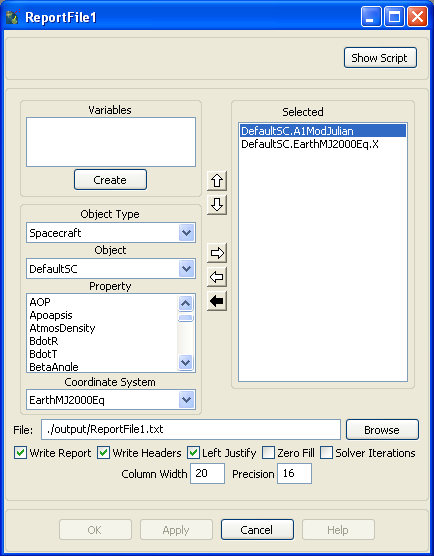
\includegraphics[%
  clip,
  scale=0.5]{./graphics/ParameterSubpanel.jpg}}}


\caption{\label{figure:ParameterSubpanel}The Updated Parameter Subpanel}
\end{figure}


The propagator subsystem needs information about the global origin
for the forces in a force model. Figure \ref{figure:PropPanelUpdate}
shows one way to add this data to the panel.

%
\begin{figure}
\centerline{\fbox{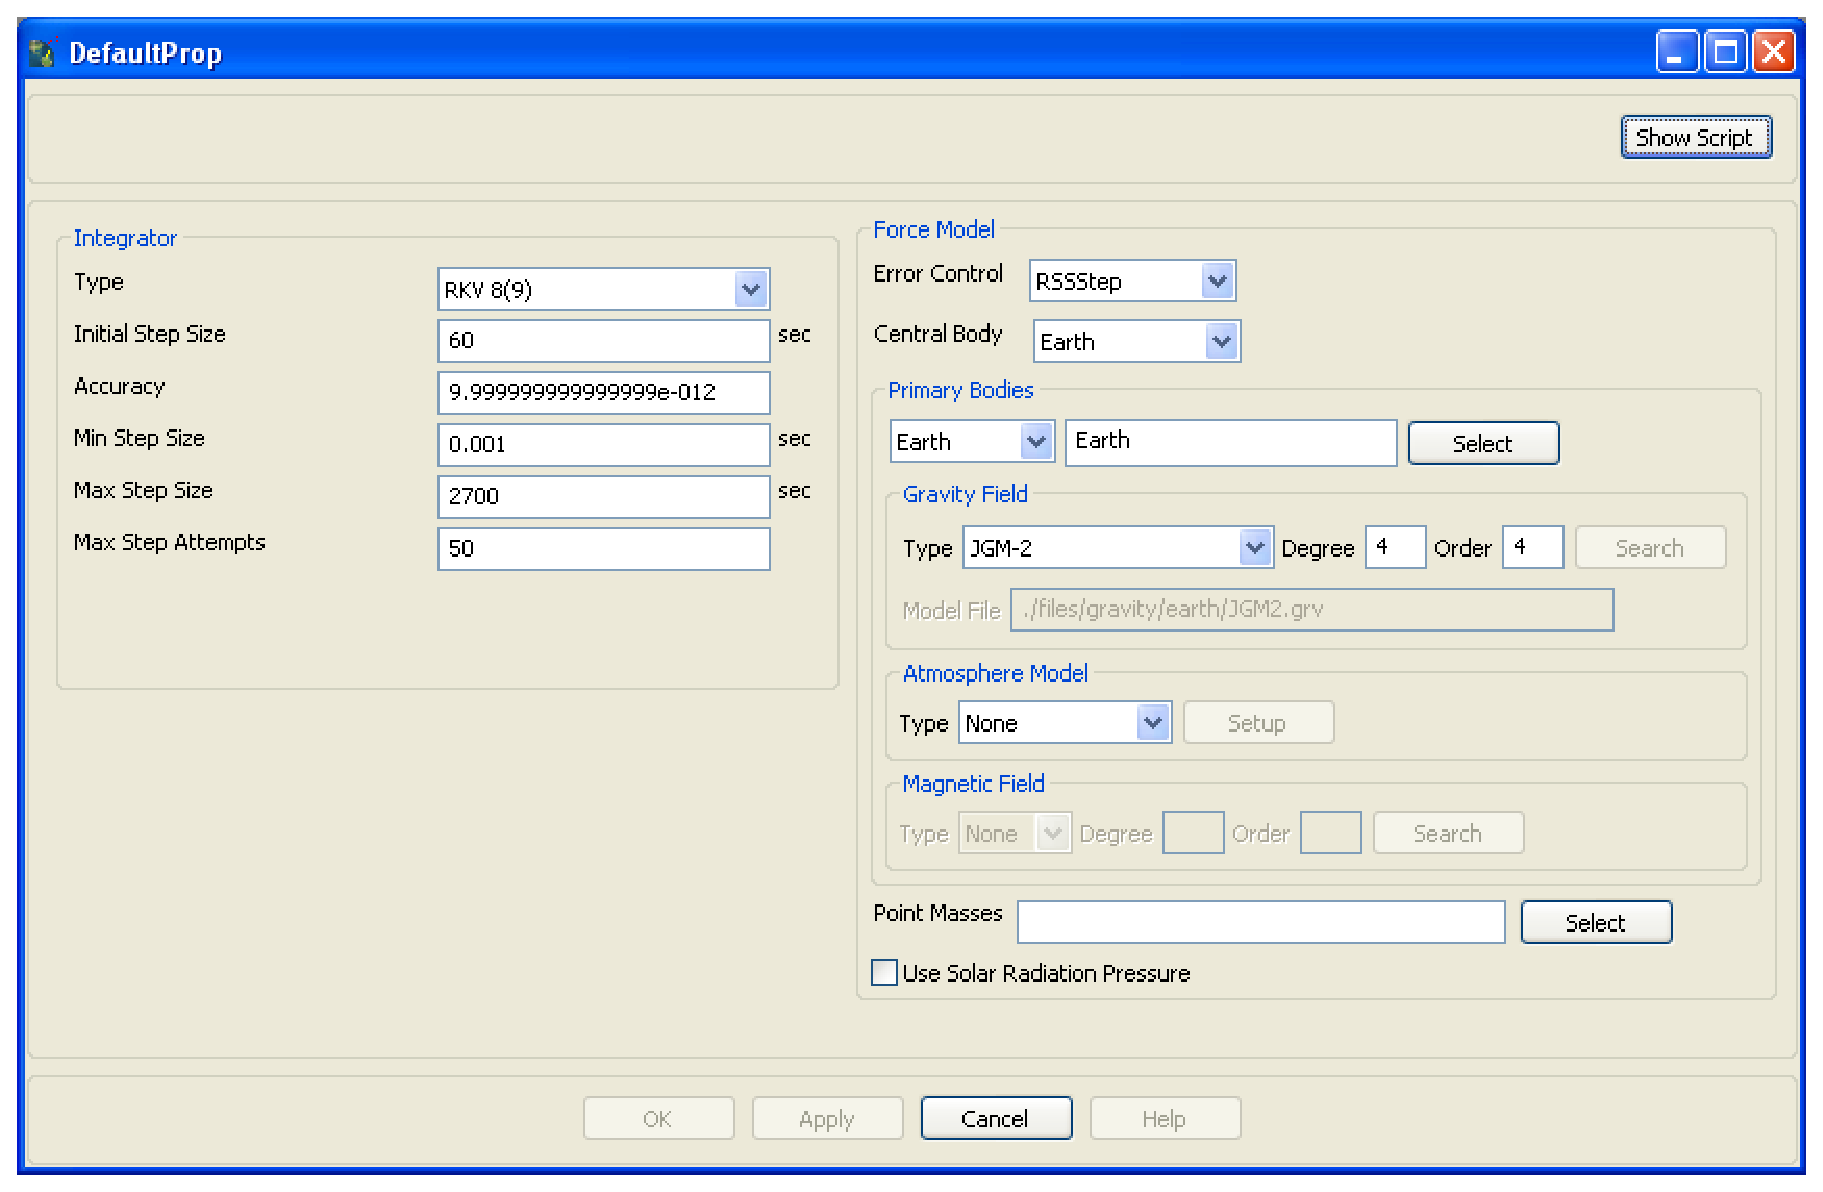
\includegraphics[%
  scale=0.5]{./graphics/PropPanel.jpg}}}


\caption{\label{figure:PropPanelUpdate}Addition of the Propagation Origin}
\end{figure}


The OpenGL panel needs to be updated to allow configuration of the
capabilities described in Section \ref{sub:OpenGLViewPoints}. Users
can use the settings on this panel to specify both the coordinate
system used to plot the mission data and the location and orientation
of the viewpoint used to observe these data. In some cases, the viewpoint
will not be a fixed point in space -- for example, users will be able
to view a spacecraft's environment in the simulation by specifying
the location and orientation of the viewpoint relative to the spacecraft
in a spacecraft centered coordinate system, and thus observe how other
objects move in relation to that spacecraft.


\section{Validation}

In this section, several tables are presented that show the data for
a single state in several different coordinate systems. GMAT tests
will be run that transform between these systems and validates taht
the conversions are in agreement with the data in the tables to an
acceptable level of precision. The test data were generated in Astrogator
by GSFC, Code 595. This output should be in agreement with GMAT results
to at least one part in $10^{12}$. (Subject to change once tests
are run -- seems like a good value as a starting point.)


\subsection{Tests for a LEO}

Table \ref{table:LEOTests} lists the expected state data for a spacecraft
orbiting near the Earth.

%
\begin{table}

\caption{\label{table:LEOTests}Coordinate Conversions for an orbit near the
Earth}

\centerline{\begin{sideways}
\begin{tabular}{|p{1.4in}|c|c|c|c|c|c|}
\hline 
\multicolumn{7}{|c|}{\textbf{A LEO State}}\tabularnewline
\hline
\hline 
\textbf{Epoch:}&
\multicolumn{2}{c|}{UTC Gregorian}&
\multicolumn{2}{c|}{UTC Julian}&
\multicolumn{2}{c|}{Ephemeris Time}\tabularnewline
\hline
\hline 
&
\multicolumn{2}{c|}{1 Jan 2005 12:00:00.00}&
\multicolumn{2}{c|}{2453372}&
\multicolumn{2}{c|}{2453372.00074287}\tabularnewline
\hline
\hline 
\textbf{Coordinate System}&
\textbf{X}&
\textbf{Y}&
\textbf{Z}&
$V_{x}$&
$V_{y}$&
$V_{z}$\tabularnewline
\hline
\hline 
{\footnotesize Earth Centered Mean J2000 Equator}&
{\footnotesize 15999.999999999998}&
{\footnotesize 0.0000000000000}&
{\footnotesize 0.0000000000000}&
{\footnotesize 0.0000000000000}&
{\footnotesize 3.8662018270519716}&
{\footnotesize 3.8662018270519711}\tabularnewline
\hline 
{\footnotesize Earth Centered Fixed}&
{\footnotesize 3100.7006422193112}&
{\footnotesize 15696.674760971226}&
{\footnotesize 7.54822029656669}&
{\footnotesize -2.6485022470204602}&
{\footnotesize 0.5213224286561129}&
{\footnotesize 3.8663431768510996}\tabularnewline
\hline 
{\footnotesize Earth Centered Mean Ecliptic of Date}&
{\footnotesize 15999.988100569937}&
{\footnotesize 19.513619701949061}&
{\footnotesize 0.0163246416692983}&
{\footnotesize -0.0062037647908650}&
{\footnotesize 5.0850309969931660}&
{\footnotesize 2.0093417847447261}\tabularnewline
\hline 
{\footnotesize Earth Centered Mean Ecliptic of J2000}&
{\footnotesize 15999.999999999998}&
{\footnotesize 0.0000000000000}&
{\footnotesize 0.0000000000000}&
{\footnotesize 0.0000000000000}&
{\footnotesize 5.0850575916827729}&
{\footnotesize 2.0092840576358051}\tabularnewline
\hline 
{\footnotesize Earth Centered Mean of Date }&
{\footnotesize 15999.9881005699370}&
{\footnotesize 17.8969907643261870}&
{\footnotesize 7.7768465297859297}&
{\footnotesize -0.0062037647908650}&
{\footnotesize 3.8661983573941092}&
{\footnotesize 3.8662003193814876}\tabularnewline
\hline
\end{tabular}
\end{sideways}}
\end{table}



\subsection{Tests for a Libration Point State}

Table \ref{table:L2Tests} lists the expected state data for a spacecraft
flying near the Earth-Sun.

%
\begin{table}

\caption{\label{table:L2Tests}Coordinate Conversions for an orbit near the
Earth/Moon-Sun L2 Point}

\centerline{\begin{sideways}
\begin{tabular}{|p{1.25in}|c|c|c|c|c|c|}
\hline 
\multicolumn{7}{|c|}{\textbf{A L2 State}}\tabularnewline
\hline
\hline 
\textbf{Epoch:}&
\multicolumn{2}{c|}{UTC Gregorian}&
\multicolumn{2}{c|}{UTC Julian}&
\multicolumn{2}{c|}{Ephemeris Time}\tabularnewline
\hline
\hline 
&
\multicolumn{2}{c|}{25 Sep 2003 16:22:47.94}&
\multicolumn{2}{c|}{2452908.18249931}&
\multicolumn{2}{c|}{2452908.18324218}\tabularnewline
\hline
\hline 
\textbf{Coordinate System}&
\textbf{X}&
\textbf{Y}&
\textbf{Z}&
$V_{x}$&
$V_{y}$&
\textbf{$V_{z}$}\tabularnewline
\hline
\hline 
{\footnotesize Earth Centered Mean J2000 Equator}&
{\footnotesize 1152413.9609139508}&
{\footnotesize 164482.90400985131}&
{\footnotesize -270853.37069837836}&
{\footnotesize -0.0237491328055502}&
{\footnotesize 0.5463496092937017}&
{\footnotesize 0.1896952705370667}\tabularnewline
\hline 
{\footnotesize Sun-Earth/Moon Barycenter L1}&
{\footnotesize 2659568.8530356660}&
{\footnotesize -467.97516783879695}&
{\footnotesize -314259.10186388291}&
{\footnotesize -0.0062197634008832}&
{\footnotesize 0.3610507604664427}&
{\footnotesize -0.0425806711166933}\tabularnewline
\hline 
{\footnotesize Sun-Earth L2}&
{\footnotesize -352659.29964214563}&
{\footnotesize -0.0002161438986659}&
{\footnotesize -313927.71991658572}&
{\footnotesize 0.0027515868356648}&
{\footnotesize 0.3488514802312706}&
{\footnotesize -0.0432916179713184}\tabularnewline
\hline 
{\footnotesize Solar System Barycenter Mean J2000 Earth Equator}&
{\footnotesize 151524360.68432158}&
{\footnotesize 4848014.2434389694}&
{\footnotesize 1751879.7152567047}&
{\footnotesize -1.6146582474186386}&
{\footnotesize 27.776726415749529}&
{\footnotesize 11.995657174332731}\tabularnewline
\hline
\end{tabular}
\end{sideways}}
\end{table}



\subsection{Tests for an Earth-Trailing State}

Table \ref{table:EarthTrailingTests} lists the expected state data
for a deep space object trailing behind the Earth.

%
\begin{table}

\caption{\label{table:EarthTrailingTests}Coordinate Conversions for an Earth-Trailing
state}

\centerline{\begin{sideways}
\begin{tabular}{|p{1.25in}|c|c|c|c|c|c|}
\hline 
\multicolumn{7}{|c|}{\textbf{An Earth-Trailing State}}\tabularnewline
\hline
\hline 
\textbf{Epoch:}&
\multicolumn{2}{c|}{UTC Gregorian}&
\multicolumn{2}{c|}{UTC Julian}&
\multicolumn{2}{c|}{Ephemeris Time}\tabularnewline
\hline
\hline 
&
\multicolumn{2}{c|}{1 Jan 2012 00:00:00.00}&
\multicolumn{2}{c|}{2455927.5}&
\multicolumn{2}{c|}{2455927.50074287}\tabularnewline
\hline
\hline 
\textbf{Coordinate System}&
\textbf{X}&
\textbf{Y}&
\textbf{Z}&
$V_{x}$&
$V_{y}$&
$V_{z}$\tabularnewline
\hline
\hline 
{\footnotesize Earth Centered Mean J2000 Equator}&
{\footnotesize 18407337.2437560}&
{\footnotesize 146717552.364272}&
{\footnotesize 2436998.6080801622}&
{\footnotesize -29.85775713588113}&
{\footnotesize 3.7988731566283533}&
{\footnotesize -0.0883535323140749}\tabularnewline
\hline 
{\footnotesize Earth Centered Mean Ecliptic of Date}&
{\footnotesize 18010745.506277718}&
{\footnotesize 135634904.81496251}&
{\footnotesize -56121251.238084592}&
{\footnotesize -29.8677194647804920}&
{\footnotesize 3.3629312165175098}&
{\footnotesize -1.5921471032003145}\tabularnewline
\hline 
{\footnotesize Earth Centered Mean Ecliptic of J2000}&
{\footnotesize 18407337.2437560}&
{\footnotesize 135580104.86024788}&
{\footnotesize -56124988.196549937}&
{\footnotesize -29.8577571358811300}&
{\footnotesize 3.4502529604822207}&
{\footnotesize -1.5921677410083135}\tabularnewline
\hline 
{\footnotesize Solar System Barycenter Mean J2000 Earth Equator}&
{\footnotesize -7095223.559007301}&
{\footnotesize 279535881.30854195}&
{\footnotesize 60015670.739229225}&
{\footnotesize -59.6890476068945470}&
{\footnotesize -0.969033406060170}&
{\footnotesize -2.1549980100429815}\tabularnewline
\hline 
{\footnotesize Sun Centered Earth Equator Mean J2000}&
{\footnotesize -6610248.770514084}&
{\footnotesize 279718577.50517684}&
{\footnotesize 60095016.884433664}&
{\footnotesize -59.6964420074725410}&
{\footnotesize -0.9617072219755838}&
{\footnotesize -2.1516618821901923}\tabularnewline
\hline 
{\footnotesize Venus Centered Fixed}&
{\footnotesize 234671807.87997022}&
{\footnotesize -184530264.43020287}&
{\footnotesize -49090196.384031780}&
{\footnotesize 87.7042809962516540}&
{\footnotesize 130.412316317457850}&
{\footnotesize -3.652395853117925}\tabularnewline
\hline 
{\footnotesize Moon Centered Fixed}&
{\footnotesize -28218680.593746454}&
{\footnotesize -133515637.46513638}&
{\footnotesize -56782561.270103499}&
{\footnotesize -325.9434285713376800}&
{\footnotesize 70.716401043687014}&
{\footnotesize -2.3269361125638657}\tabularnewline
\hline 
{\footnotesize Moon Centered Inertial Moon Equator}&
{\footnotesize 18009331.473252095}&
{\footnotesize 146686558.45310178}&
{\footnotesize 2386670.4083221816}&
{\footnotesize -29.7707871076046790}&
{\footnotesize 2.8992895961634191}&
{\footnotesize -0.4430059951218515}\tabularnewline
\hline 
{\footnotesize Jupiter Centered Inertial Jupiter Equator}&
{\footnotesize -562256455.23257434}&
{\footnotesize -225513430.99244595}&
{\footnotesize -25746106.471387718}&
{\footnotesize -50.5813599808322610}&
{\footnotesize -13.854862630504574}&
{\footnotesize -0.5555336109134552}\tabularnewline
\hline 
{\footnotesize Mars Centered Inertial Mars Equator}&
{\footnotesize 207783148.71266919}&
{\footnotesize -43368297.655312374}&
{\footnotesize 13161295.341311477}&
{\footnotesize -19.7427310285643220}&
{\footnotesize 35.2164929323613260}&
{\footnotesize -21.767269119097524}\tabularnewline
\hline 
{\footnotesize Mars Centered Fixed}&
{\footnotesize 127577563.32704885}&
{\footnotesize -169644368.24313599}&
{\footnotesize 13138473.444519326}&
{\footnotesize -12016.3787728729480}&
{\footnotesize -9003.4840556769759}&
{\footnotesize -21.769072220711045}\tabularnewline
\hline
\end{tabular}
\end{sideways}}
\end{table}



\section{Some Mathematical Details}

\textbf{This section will probably appear in some form in the mathematical
specifications. I'm leaving it here until I can confirm that assumption.}

A spatial coordinate system is fully specified by defining the origin
of the system and two orthogonal directions. Given these pieces of
data, space can be gridded into triplets of numbers that uniquely
identify each point. The purpose of this section is to provide some
guidance into how to proceed with the definition of the coordinate
system axes once the origin and two directions are specified.


\subsection{Defining the Coordinate Axes}

The coordinate system axes are defined from the two orthogonal directions
in the system specification. These directions are given two of the
three labels $\hat{X}$, $\hat{Y}$, and $\hat{Z}$. These labels
are used to define the corresponding directions for the coordinate
system. The third axis is calculated by taking the inner product of
the other two axes, using \begin{eqnarray}
\hat{X} & = & \hat{Y}\times\hat{Z}\nonumber \\
\hat{Y} & = & \hat{Z}\times\hat{X}\nonumber \\
\hat{Z} & = & \hat{X}\times\hat{Y}\label{eq:UnitVectorTriplets}\end{eqnarray}



\subsection{Setting Directions in GMAT}

The principal directions for a coordinate system are set in GMAT by
specifying a primary direction and a secondary direction. The specified
secondary axis need not be orthogonal (i.e. perpendicular) to the
primary axis. Given a primary direction $\vec{P}$ and a secondary
direction $\vec{S}$, the primary axis is oriented along a unit vector
given by \begin{equation}
\hat{P}=\frac{\vec{P}}{\left|\vec{P}\right|}\end{equation}


The unit vector defining the secondary axis is constructed by projecting
the secondary direction $\vec{S}$ into the plane perpendicular to
the primary direction, and unitizing the resulting vector. This is
done by calculating \begin{equation}
\hat{S}=\frac{\vec{S}-\left(\vec{S}\cdot\hat{P}\right)\hat{P}}{\left|\vec{S}-\left(\vec{S}\cdot\hat{P}\right)\hat{P}\right|}\end{equation}


In general, two points are needed to specify a direction.

\begin{thebibliography}{1}
\bibitem{GmatMathSpec}S. Hughes, \textbf{Goddard Mission Analysis Tool (GMAT) Mathematical
Specifications and User's Guide}, November, 2004.
\bibitem{wxWidgets}Available from www.wxwidgets.org.
\bibitem{Vallado}D. Vallado, \textbf{Fundamentals of Astrodynamics and Applications},
2nd Ed., Microcosm Press, 2001.
\bibitem{Poseidon}\textit{Poseidon for UML}, available from www.Gentleware.com. The
Community Edition is free.
\bibitem{MATLAB}Available from www.mathworks.com. GMAT is being developed using MATLAB
7.0.\end{thebibliography}

\end{document}
